\documentclass{article}

\usepackage[utf8]{inputenc}
\usepackage[T1]{fontenc}
\usepackage[norsk,english]{babel}   %Norsk først så engelsk, så engelsk blir prioritert
\usepackage{graphicx}
\usepackage{amsmath}        %For å kunne skrive matte
\usepackage{listings}       %?????????
\usepackage{multicol}       %Importerer pakken for multikolonner til teksten
\usepackage[margin=2.54cm]{geometry}    %Definerer hva bredden til teksten er
\usepackage{wrapfig}    %Importerer pakken for å ha bildene i teksten

%Definerer hyperlinker og dens farger
\usepackage{hyperref}
\hypersetup{
    colorlinks,
    citecolor=blue,
    filecolor=black,
    linkcolor=blue,
    urlcolor=blue
}

%-----------------------------------

%Definerer farger til kodeeksemplene i PDF-en
\usepackage{color}

\definecolor{codegreen}{rgb}{0,0.6,0}
\definecolor{codegray}{rgb}{0.5,0.5,0.5}
\definecolor{codepurple}{rgb}{0.58,0,0.82}
\definecolor{backcolour}{rgb}{0.95,0.95,0.92}

\lstdefinestyle{mystyle}{
    backgroundcolor=\color{backcolour},
    commentstyle=\color{codegreen},
    keywordstyle=\color{magenta},
    numberstyle=\tiny\color{codegray},
    stringstyle=\color{codepurple},
    basicstyle=\footnotesize,
    breakatwhitespace=false,
    breaklines=true,
    captionpos=b,
    keepspaces=true,
    numbers=left,
    numbersep=5pt,
    showspaces=false,
    showstringspaces=false,
    showtabs=false,
    tabsize=2
}

\lstset{style=mystyle}

%------------------------------------

\setlength{\parindent}{0pt} %Ingen indent automaisk for nye linjer
%\setlength{\columnsep}{2mm} %Column separation - til multicolumn

%\setlength{\arrayrulewidth}{1mm}   %Hvilken tykkelse tabellene skal ha
\setlength{\tabcolsep}{3mm}     %Lengden mellom hver kolonne
\renewcommand{\arraystretch}{1.5}   %Hvor stor avstand det skal være mellom radene

\iffalse    %midlertidig endre bredden på teksten
If you want to change this temporarily, you can write:
\savegeometry{mydefaultgeometry}
\newgeometry{margin=3in}
And then later you can call:
\loadgeometry{mydefaultgeometry}
\fi

%for å fjerne overskriften "refrences" som kommer automatisk når man bruker bibtex
\usepackage{etoolbox}
\patchcmd{\thebibliography}{\section*{\refname}}{}{}{}

%----------------------------------------------------------------------------------------

\begin{document}

\addtocounter{page}{0}

\title{Project 3 \\
      \large For the course FYS3150}
\date{\today \\
    \vspace{1mm}
    \large Week 40 - ??}

\author{Erik Grammeltvedt, Erlend Tiberg North and Alexandra Jahr Kolstad}

\maketitle

%\newpage

%------------Her starter skrivingen-----------------------------------------

%\begin{multicols}{2}

\newpage
\clearpage

\textbf{\Large DET er PARALLELIZED ?????????} \\

\vspace{3cm}

\textbf{Kommentarer fra project 1 på devilry:}

\begin{itemize}

\item Abstract: short motivation and presentation of the results and the findings \\

\item Introduction: you want to motive the reader about the problem and why you want solve it \\

\item Theory: explaining the theory behind the solution method and the problem \\

\item Method/implementation: how you implement the solution in order to fix/solve the problem \\

\item Results/graphs/tables: presenting the results \\

\item Discussion: Discussing the result from previous section \\

\item Conclusion: concluding the findings, your neutral opinion, etc… and future work \\

\item Appendix: How you derived your method, theory, etc… , altså utledning av ting i teori som ikke spesifikt er et bevis \\

\end{itemize}


Ting å gjøre for de ulike oppgavene:
\begin{itemize}

  \item 3a: beregne integralet, how many mesh points, lage et plott for å sjekke om grensene er passende å bruke \\

  \item 3b: finne grensene, erstatte Gauss-Legendre metoden med Laguerre polynomer, sammenligne med resultater fra a \\

  \item 3c: nå bruke brute force Monte Carlo, sammenligne resultatene med tidligere \\

  \item 3d: forbedre Monte Carlo med bruk av importance sampling, kommentere resultatene, lage en liste over tidene, sammenligne resultatene \\

  \item 3e: parallellisere koden fra 3d med openMP eller MPI, kommenter resultatene (hovedsakelig i tiden brukt)

\end{itemize}

\vspace{1cm}

\textbf{Det som mangler:}

\begin{itemize}
    \item skrive mer på introduction \\
    \item lime inn theory \\
    \item skrive noe på method \\
    \item lime inn results \\
    \item skrive discussion \\
    \item skrive conclusion and perspective \\
    \item sjekke om vi skal ha noe i appendix \\
    \item sjekke references \\
\end{itemize}


%-------------------- Abstract -------------------------------
\vspace{1cm}


\begin{center}

{\Large\textbf{Abstract}} \label{sec:Abstract}

\end{center}

\vspace{5mm}

In this scientific study we will compute an integral with different numerical methods of integration to approximate the ground state correlation energy between two electrons in a helium atom. Our integral is given by equation (\ref{eq:integral}). The integral has the analytical answer $\frac{5 \pi^2}{16^2} \approx 0.192765710958777$. The main interest and the goal of this study is to look at how the methods compare with different amount of mesh points and integration limits. The numerical integration methods we will use are Gauss-Legendre quadrature, Gauss-Laguerre quadrature, brute force Monte Carlo, spherical Monte Carlo with importance sampling, and spherical Monte Carlo with parallelization. The study was a success and proved Monte Carlo to be the fastest and most accurate method. In fact, the improved spherical Monte Carlo was $3572\times$ faster than Gauss-Laguerre in achieving an error $|\varepsilon|<0.001$. Being based on big data, it required many more sampling points. However, as it did not manually calculate the integral, it was astronomically much more efficient. \\

%All programs are found at our \href{https://github.com/Erikbgram/Fys3150}{GitHub-repository}. \\


\newpage

%------------------- Table of contents -----------------------

\vspace{1cm}

\tableofcontents

\vspace{1cm}

%-------------------- Introduction ------------------------------
\vspace{1cm}

\section{Introduction} \label{sec:Introduction}

The integral we are evaluating comes from the solution of Schrödinger's equation for a simplified case of determining the ground state correlation energy between two electrons in a helium atom.

\begin{equation} \label{eq:integral}
    \left\langle \frac{1}{| \vec{r_1} - \vec{r_2} |} \right\rangle = \int_{-\infty} ^\infty d \vec{r_1} d \vec{r_2} \hspace{1mm} e^{- 2 \alpha (r_1 + r_2)} \hspace{1mm} \frac{1}{| \vec{r_1} - \vec{r_2} |}
\end{equation} \\

The integral is not properly normalized. However, that is not important for the study. If you are interested in how the integral is found, see \cite{task}.\\

Numerical integration methods can be used to numerically solve this integral. For instance Gaussian quadrature uses orthogonal polynomials to compute weights and uses Taylor series to approximate an integral. The Gauss-Legendre method implements the theory without further thought to effectiveness. Therefore this method is called brute force Gauss-Legendre, and uses the cartesian coordinate system. An improved Gaussian quadrature rule would be based on spherical coordinates, to

Our aim is to approximate this integral using two types of Gaussian quadrature, and some variations of Monte Carlo. We have created a code that evaluates the integral using each method and compares them. Alongside the actual value we get the absolute value and time used. Using this we present our data showing that Monte Carlo massively outperforms the Gaussian quadrature rules, and especially the superiorness of the parallelized spherical Monte Carlo in computation time. \\

The study will go through the theory and methods behind our study and following that we will present our results and discuss them. Lastly we have a conclusion to briefly summarise our findings. Other findings which we deemed to not be as important are found in the appendix, for instance some calculations. Sources of different academic materials we used are given in references. \\


%-------------------- Theory ------------------------------------
\vspace{1cm}

\section{Theory} \label{sec:Theory}

\subsection{Theory of Gaussian quadrature and the Gauss-Legendre method}

The Gauss-Legendre method is based on the more general Gaussian quadrature rule which uses Taylor series to solve an integral. The main idea is to generate weights, by solving sets of linear equations. For $N$ points in the Taylor series we get $N$ weights. These weights are used in a weight function in order to approximate the integral. The theory behind Gaussian quadrature is to obtain the weights by using orthogonal polynomials. These polynomials are orthogonal in certain intervals. For instance for $[3,7]$, we can use these orthogonal polynomials in order to ensure a smooth integral for our graph. The $x_i$ values are chosen arbitrary within the given interval. Together with the weights this gives us $2N$ parameters that can be used to solve the integral. \\

\begin{equation} \label{eq:integralgauleg}
    I = \int_{a}^{b} f(x) = \int_{a}^{b}W(x)g(x) \hspace{1mm} dx \approx  \sum_{n=1}^{N}  \omega_i g(x_i)
\end{equation} \\

In equation (\ref{eq:integralgauleg}) we have the weight function $W(x)$ and $g(x)$ is an orthogonal polynomial that gives a smooth graph. Then we have the sum of the weights, $\omega_i$, and the orthogonal polynomial $g(x_i)$ with a number of $x_i$ values within the given interval. \\

In order to go from Gaussian quadrature to the Gauss-Legendre method a unit change is needed. Because the Gauss-Legendre method uses only the integral from $[-1,1]$ and later apply the Gaussian quadrature, we have to implement a unit change. The unit change is given by the change of $t$ to $t = \frac{b-a}{2}x + \frac{a+b}{2}$. Our integral can now be written as \\

\begin{equation} \label{eq:tchangeintegralgauleg}
    \int_{a}^{b} f(t) \hspace{1mm} dt = \frac{b-a}{2}\int_{-1}^{1} f \left( \frac{b-a}{2}x + \frac{a+b}{2} \right) \hspace{1mm} dx
\end{equation} \\

Now inserting this new integral, (\ref{eq:tchangeintegralgauleg}), into the Gaussian quadrature, (\ref{eq:integralgauleg}), the following estimate of the integral becomes equation (\ref{eq:finalintegralgauleg}). \\

\begin{equation} \label{eq:finalintegralgauleg}
    \int_{a}^{b} f(t) \hspace{1mm} dt \approx \frac{b-a}{2} \sum_{n=1}^{N} \omega_i f \left( \frac{b-a}{2}x + \frac{a+b}{2} \right) \hspace{1mm} dx
\end{equation} \\

\subsection{Theory of the Montecarlo Method}


%--------------------- Method ------------------------------------
\vspace{1cm}

\section{Method} \label{sec:Method}


THIS SHOULD ALSO BE ERIK SITT?

%--------------------- Results ----------------------------------
\vspace{1cm}

\section{Results} \label{sec:Results}

  \textit{Our results are as shown in the \nameref{sec:Appendix}}. We also have \texttt{.txt}-files for all the raw data generated by the projects up on \href{https://github.com/Erikbgram/Fys3150}{GitHub}. \\

\begin{itemize}

  \item How many mesh points do you need before the results converges at the level of the third leading digit?

  \item plottene for lambda, integrationspoints, montecarlo og timings

  \item tror ikke skal ha noen tabeller

\end{itemize}

  Burde ha at lambda er 2 siden det gir best resultater, se plottet fra plot\_data.txt.


  \begin{figure}[ht]
  	\centering
    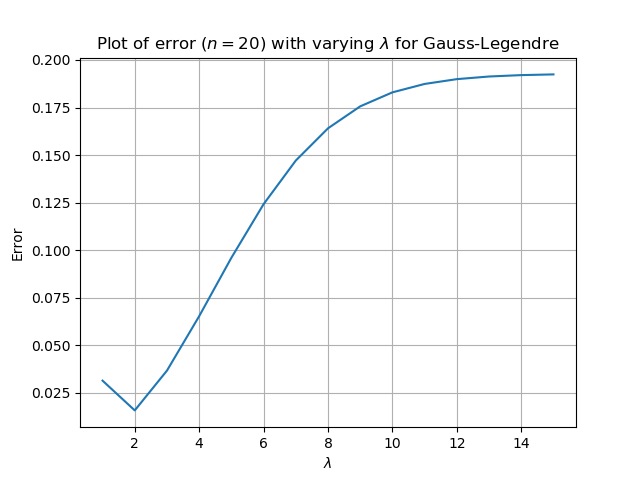
\includegraphics[width = 11cm]{images/error-lambda.png}
  	\caption{The plot of error as a function of lambda for Gauss-Legendre. }
    \label{fig:lambdapng}
  \end{figure}

  \begin{figure}[ht]
    \centering
    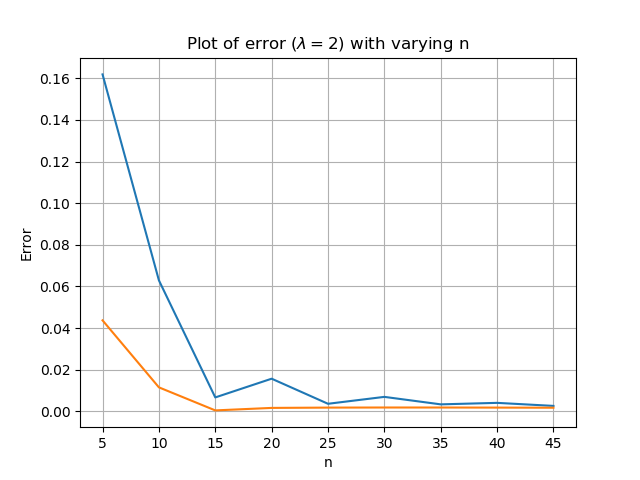
\includegraphics[width = 11cm]{images/error-integrationpoints.png}
    \caption{The plot of error as a function of integrations points $n$ for Gauss-Legendre and Gauss-Laguerre. }
    \label{fig:integrationpointspng}
  \end{figure}

  \begin{figure}[ht]
    \centering
    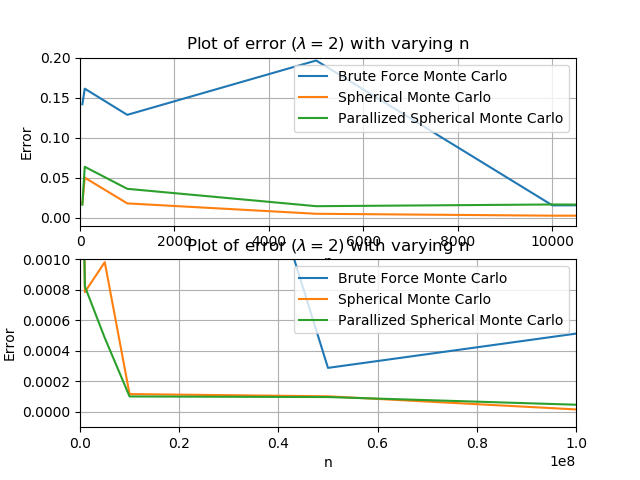
\includegraphics[width = 11cm]{images/error-montecarlo.png}
    \caption{The plot of error as a function of integration points $n$ for brute force Monte Carlo, spherical Monte Carlo with importance sampling, and parallelized spherical Monte Carlo with importance sampling. }
    \label{fig:montecarlopng}
  \end{figure}

\begin{table}[ht]
    \centering
    \caption{Error and time for Gauss-Legendre as a function of $\lambda$ with the set value $n = 20$. }
    \vspace{2mm}
    \label{tab:lambda}
    \begin{tabular}{|c|c|c|c|}
        \hline
        $n$ & $\lambda$ & error & time \\
        \hline \hline
        20 & 1 & 0.0313459 & 3.35521 \\
        20 & 2 & 0.0157005 & 3.32988 \\
        20 & 3 & 0.0366263 & 3.33241 \\
        20 & 4 & 0.0652528 & 3.34317 \\
        20 & 5 & 0.0959769 & 3.33531 \\
        20 & 6 & 0.124165 & 3.33762 \\
        20 & 7 & 0.147104 & 3.33286 \\
        20 & 8 & 0.164053 & 3.34689 \\
        20 & 9 & 0.175608 & 3.33201 \\
        20 & 10 & 0.182966 & 3.33199 \\
        20 & 11 & 0.187388 & 3.3834 \\
        20 & 12 & 0.189917 & 3.41952 \\
        20 & 13 & 0.191303 & 3.33239 \\
        20 & 14 & 0.192035 & 3.32912 \\
        20 & 15 & 0.192409 & 3.47462 \\
        \hline
      \end{tabular} \\
      \hspace{0pt}\\
  \end{table}

  \begin{table}[ht]
    \centering
    \caption{Error and execution time for Gauss-Legendre and Gauss-Laguerre.}
    \vspace{2mm}
    \label{tab:error-gauss}
    \begin{tabular}{|c|c|c|c|c|c|}
        \hline
        $n$ & $\lambda$ & Legendre error & Laguerre error & Legendre time & Laguerre time   \\
        \hline \hline
        5 & 2 & 0.161836 & 0.0437248 & 0.00082727 & 0.0022169 \\
        10 & 2 & 0.0629315 & 0.0115411 & 0.0520311 & 0.150486 \\
        15 & 2 & 0.00670907 & 0.000476827 & 0.609131 & 1.69456 \\
        20 & 2 & 0.0157005 & 0.00167232 & 3.35013 & 9.3416 \\
        25 & 2 & 0.00365618 & 0.00181852 & 12.8663 & 35.5266 \\
        30 & 2 & 0.00697009 & 0.00186703 & 38.0615 & 105.708 \\
        35 & 2 & 0.00337855 & 0.00186074 & 95.5971 & 264.104 \\
        40 & 2 & 0.00409558 & 0.00181934 & 214.105 & 608.182 \\
        45 & 2 & 0.00263748 & 0.00176034 & 433.725 & 1191.8 \\
        50 & 2 & 0.00281127 & 0.00169433 & 831.449 & 2314.1 \\
        \hline
    \end{tabular} \\
    \hspace{0pt}\\
  \end{table}

  \begin{table}[ht]
    \centering
    \caption{Error and execution time for brute force Monte Carlo, spherical Monte Carlo with importance sampling, and parallelized spherical Monte Carlo with importance sampling.}
    \vspace{2mm}
    \label{tab:error-montecarlo}
    \begin{tabular}{|c|c|c|c|c|c|c|c|}
        \hline
        $n$ & $\lambda$ & BMC error & SMC error & PSMC error & BMC time & SMC time & PSMC time  \\
        \hline \hline
        50 & 2 & 0.138417 & 0.251552 & 0.131809 & 0.00011814 & 8.7853e-05 & 0.00038 \\
        100 & 2 & 0.157825 & 0.156198 & 0.0071997 & 0.00014777 & 0.0001193 & 0.00037 \\
        500 & 2 & 0.113224 & 0.012164 & 0.00302251 & 0.0003764 & 0.0003822 & 0.00051 \\
        1000 & 2 & 0.079204 & 0.0168798 & 0.022215 & 0.00066215 & 0.0007048 & 0.00098 \\
        5000 & 2 & 0.029304 & 0.011712 & 0.013536 & 0.0029481 & 0.00338986 & 0.002612 \\
        10000 & 2 & 0.0457817 & 0.00027297 & 0.018113 & 0.005808 & 0.006558 & 0.005258 \\
        50000 & 2 & 0.0096648 & 0.0038374 & 0.0012646 & 0.029013 & 0.032508 & 0.025366 \\
        100000 & 2 & 0.024003 & 0.0043587 & 0.00030587 & 0.056982 & 0.067961 & 0.047938 \\
        500000 & 2 & 0.0137398 & 0.0046188 & 0.00356363 & 0.287352 & 0.328019 & 0.18964 \\
        1000000 & 2 & 0.0161491 & 0.00049579 & 0.0005530 & 0.57400 & 0.654257 & 0.354581 \\
        5000000 & 2 & 0.00311977 & 0.00048176 & 0.00026134 & 2.85616 & 3.27695 & 1.82245 \\
        10000000 & 2 & 0.00481115 & 0.00012881 & 2.40583e-05 & 5.70269 & 6.54182 & 3.3623 \\
        50000000 & 2 & 0.00265522 & 9.08138e-05 & 5.988e-05 & 29.7091 & 33.0613 & 16.5097 \\
        100000000 & 2 & 0.00117823 & 0.0001726 & 7.16594e-05 & 58.8054 & 67.2903 & 33.4236 \\
        500000000 & 2 & 6.0793e-05 & 2.5923e-05 & 1.6625e-05 & 415.953 & 448.229 & 208.211 \\
        \hline
    \end{tabular} \\
    \hspace{0pt}\\
  \end{table}




%--------------- Discussion ---------------------------------------
\vspace{1cm}

\section{Discussion} \label{sec:Discussion}

diskutere resultatetene: altså hvilke metoder som brukte lengst tid, hvilke som var mest nøyaktig osv \\
koble dette til teori for hvorfor resultatene ble slik som de er \\

Both Gauss-Legendre and brute force Monte Carlo use $\lambda$ as a parameter for the integration limits. Looking at table (\ref{tab:lambda}) we can see how the accuracy of Gauss-Legendre depends on the value of $\lambda$. We see that the time is more or less constant (as it should be), and that $\lambda=2$ works best. A too small $\lambda$ will give an evaluation of a too small area of the wave-function. A too large $\lambda$ won't give a large improvement (since the wave-function goes to zero after a certain length). In fact, since $\lambda$ increases the distance between the mesh points will increase, resulting in reduced accuracy.

By looking at table (\ref{tab:error-gauss}) we see that Gaussian quadrature improves greatly by increasing the amount of mesh points, at least for smaller $n$. When we pass about $n=30$ we start getting diminishing returns. The calculation starts taking a very long time, and the improvement in error is not as great as it was for smaller values. \\

Monte Carlo is a data-hungry method, and as such, it requires a lot of data points. Looking at table (\ref{tab:error-montecarlo}) we see that it is not great at the same values of $n$ as Gaussian quadrature. At the same time, it is easy to see that Monte Carlo is much faster. Only on values for $n=50000000$ and beyond, Monte Carlo starts struggling. After implementing parallelization the code also also sped up  by a factor of the machine's available cores (2 in our case).\\

The results show that the parallelized code actually isn't better than the non-parallelized code. This is strange. However, it can be attributed to the fact that the computer running the code only has two cores, meaning there is less of an effect. In addition, there is always the possibility of some mistake in the code. We also divided the element of each sum by took the average of the to cores results, instead of dividing each element in the sum by $n_{total}$

%---------------Conclusion and perspective---------------------------
\vspace{1cm}

\section{Conclusion and perspective} \label{sec:Conclusion}

To conclude the Monte Carlo integration methods exceeded the Gaussian quadrature methods for both computation time and accuracy of the answer to the integral. As expected the parallelized spherical Monte Carlo with importance sampling is the fastest method with the highest degree of accuracy. This is mainly because ... \\

legge inn mer her som knytter det opp til teorien.


%--------------Appendix---------------------------------------------
\vspace{1cm}

\section{Appendix} \label{sec:Appendix}

\subsection{Calculation of Monte Carlo's speed over Gauss-Laguerre}
We imported the error as function of time for SMC and Gauss-Laguerre into Geogebra and did a simple regression analysis. For both data-sets, the $f(x)=Cx^p$ was the best fit. By extrapolating to $error=0.001$ we found SMC to intersect at $0.639487186$ and Gauss-Laguerre to intersect at
$2284.1372326374$. Dividing Laugerre with SMC, we found SMC to be $3571.82643$ times faster. Approximately $3572$ times faster. This seems crazy high, so we
have also included the calculation for the actual time for the 1st run where Laugerre and SMC went below $error=0.001$. See below.\\

The 1st time improved Monte Carlo (spherical) achieved an absolute error below $0.001$ was with $n=10000$. The error was $0.000272967$ and it took
$0.00655811$ seconds. The 1st time Gauss-Laguerre (improved Gaussian quadrature) achieved an absolute error below $0.001$ was with $n=15$. The error was $0.000476827$ and it took $1.69456$ seconds. \\

Calculation follows: \\

$$\frac{time_{Laguerre}}{time_{SMC}} = \frac{1.69456}{0.00655811} = 258.3915183$$ \\

Spherical Monte Carlo was approximately $258$ times faster than Gauss-Laguerre.\\

Figure (\ref{fig:timingslargepng}) does not include all larger data points from our \texttt{.txt}-files. These can be found in table (\ref{tab:error-montecarlo}) for the latter rows. These values can also be found in the file \texttt{montecarlo.txt} on our GitHub, \cite{github}.

\begin{figure}[ht]
    \centering
    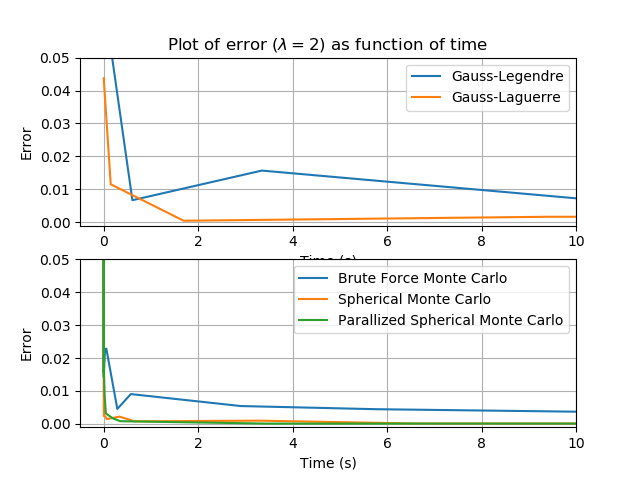
\includegraphics[width = 11cm]{images/method-timings-small.png}
    \caption{The plot of error as a function of time for all the numerical integration methods used in this scientific study. }
    \label{fig:timingssmallpng}
\end{figure}

\begin{figure}[ht]
    \centering
    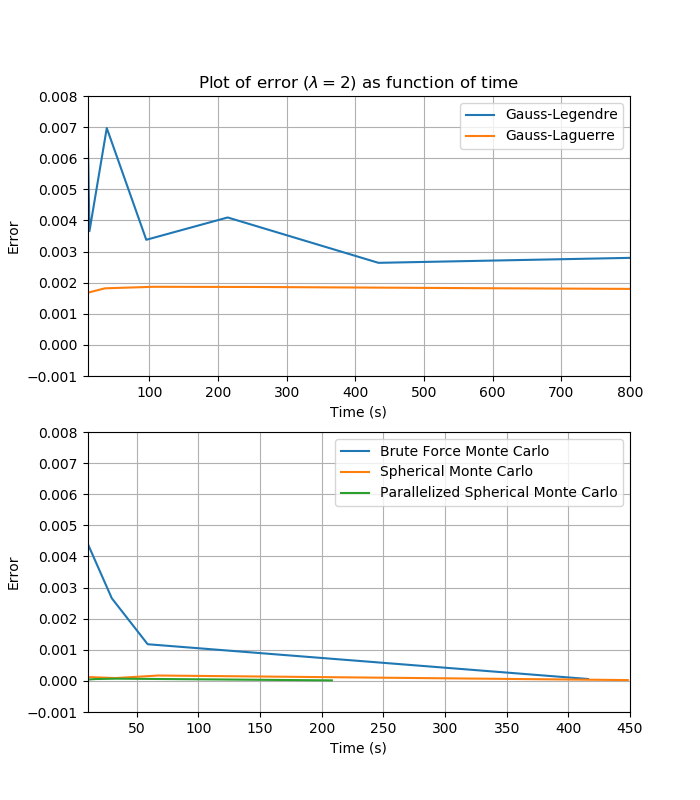
\includegraphics[width = 11cm]{images/method-timings-large.png}
    \caption{This figure is a continuation of the previous figure, (\ref{fig:timingssmallpng}). }
    \label{fig:timingslargepng}
\end{figure}


%\clearpage

%----------------References----------------------------------------
\vspace{1cm}

\section{References} \label{sec:References}

\begin{thebibliography}{}

\bibitem{task}
Morten H. Jensen (2019), \href{https://github.com/CompPhysics/ComputationalPhysics/blob/master/doc/Projects/2019/Project3/pdf/Project3.pdf}{Project 3}, Departement of Physics, University of Oslo, Norway

\bibitem{github}
Erik B. Grammeltvedt, Alexandra Jahr Kolstad, Erlend T. North (2019), \href{https://github.com/Erikbgram/Fys3150}{GitHub}, Students of Departement of Physics, University of Oslo, Norway

\bibitem{lecture_slides}
Morten H. Jensen (2015), \href{https://github.com/CompPhysics/ComputationalPhysics/blob/master/doc/Lectures/lectures2015.pdf}{Lecture slides for FYS3150}, Department of Physics, University of Oslo, Norway

\bibitem{laguerre_polynomial}
Weisstein, Eric W. \href{http://mathworld.wolfram.com/LaguerrePolynomial.html}{"Laguerre Polynomial."}, From MathWorld--A Wolfram Web Resource. 

\end{thebibliography}


%----------------Slutten av dokumentet---------------------------------------


%\end{multicols}

\end{document}
